\documentclass[compress]{beamer}
\usepackage{ifthen,verbatim}

\newcommand{\isnote}{}
\xdefinecolor{lightyellow}{rgb}{1.,1.,0.25}
\xdefinecolor{darkblue}{rgb}{0.1,0.1,0.7}

%% Uncomment this to get annotations
%% \def\notes{\addtocounter{page}{-1}
%%            \renewcommand{\isnote}{*}
%% 	   \beamertemplateshadingbackground{lightyellow}{white}
%%            \begin{frame}
%%            \frametitle{Notes for the previous page (page \insertpagenumber)}
%%            \itemize}
%% \def\endnotes{\enditemize
%% 	      \end{frame}
%%               \beamertemplateshadingbackground{white}{white}
%%               \renewcommand{\isnote}{}}

%% Uncomment this to not get annotations
\def\notes{\comment}
\def\endnotes{\endcomment}

\setbeamertemplate{navigation symbols}{}
\setbeamertemplate{headline}{\mbox{ } \hfill
\begin{minipage}{5.5 cm}
\vspace{-0.75 cm} \small
\end{minipage} \hfill
\begin{minipage}{4.5 cm}
\vspace{-0.75 cm} \small
\begin{flushright}
\ifthenelse{\equal{\insertpagenumber}{1}}{}{Jim Pivarski \hspace{0.2 cm} \insertpagenumber\isnote/\pageref{numpages}}
\end{flushright}
\end{minipage}\mbox{\hspace{0.2 cm}}\includegraphics[height=1 cm]{../cmslogo} \hspace{0.1 cm} \includegraphics[height=1 cm]{../tamulogo} \hspace{0.01 cm} \vspace{-1.05 cm}}

\newcommand{\s}[1]{{\mbox{\scriptsize #1}}}

\begin{document}
\begin{frame}
\vfill
\begin{center}
\textcolor{darkblue}{\Large GlobalMuon/HLT efficiency for close-by muons}

\vfill
\begin{columns}
\column{0.3\linewidth}
\begin{center}
\large
Jim Pivarski
\end{center}
\end{columns}

\begin{columns}
\column{0.3\linewidth}
\begin{center}
\scriptsize
{\it Texas A\&M University}
\end{center}
\end{columns}

\vfill
 4 October, 2010

\end{center}
\end{frame}

%% \begin{notes}
%% \item This is the annotated version of my talk.
%% \item If you want the version that I am presenting, download the one
%% labeled ``slides'' on Indico (or just ignore these yellow pages).
%% \item The annotated version is provided for extra detail and a written
%% record of comments that I intend to make orally.
%% \item Yellow notes refer to the content on the {\it previous} page.
%% \item All other slides are identical for the two versions.
%% \end{notes}

\small

%% \begin{frame}
%% \frametitle{Motivation}

%% \vspace{0.4 cm}
%% \hfill \includegraphics[height=3.5 cm]{eventdisplay_3d.pdf}

%% \vspace{-3.9 cm}
%% \begin{itemize}
%% \item Physics searches for new low-mass, high- \\ momentum resonances
%%   decaying to muons \\ (``lepton jets'') will need to be able to \\
%%   reconstruct and trigger on muons that pass \\ close to each other in
%%   the muon system

%% \item This case is distinct from $J/\psi$ reconstruction: \\
%%   lepton jet models typically predict groups of \\ muons with tens to hundreds of GeV/$c$

%% \item Low-momentum muons can ``get away from each other'' by curving
%%   in the $\vec{B}$-field; high-momentum muons have a greater potential
%%   for overlap in the muon system and therefore lower efficiencies
%% \end{itemize}

%% \vspace{0.1 cm}
%% \hspace{-0.83 cm} \textcolor{darkblue}{\Large This talk}
%% \begin{itemize}
%% \item MC dimuon pair-gun study to find and \mbox{quantify regions of inefficiency\hspace{-1 cm}}

%% \item There are large inefficiencies in the StandAloneMuon-building step

%% \item Observed in HLT as well (which are based on GlobalMuons)
%% \end{itemize}
%% \end{frame}

\begin{frame}
\frametitle{Reminder of method}
\begin{columns}
\column{0.52\linewidth}
\begin{itemize}
\item Generated a sample of dimuons with uniformly distributed mass:
  $2m_\mu$--50~GeV/$c^2$ (each dimuon has a different mass) and
  pair-$p_T$: 0--100~GeV/$c$

\item Not a realistic physics process: the point is to find variables
  that quantify nearby-muon efficiency in a model-independent way

\item First, detector-based variables: propagate generator-level muons
  to the muon system and plot efficiency as a function of
\begin{itemize}
\item $\Delta \phi$ and $\Delta z/r$ on a cylinder with $r=600$~cm
\item $\Delta \phi$ and $\Delta r/z$ on a plane with $z=700$~cm
\end{itemize}
\end{itemize}

\column{0.5\linewidth}
\centering
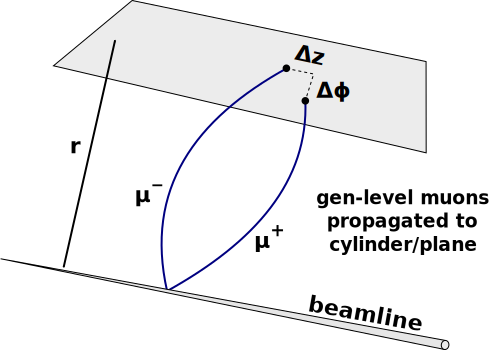
\includegraphics[width=0.7\linewidth]{propagations.pdf}

\vspace{0.5 cm}
\mbox{Cylinder for $|\eta| < 1$, plane for $|\eta| > 1$\hspace{-0.15 cm}}

\includegraphics[width=\linewidth]{cms_quarterview.pdf}
\end{columns}
\end{frame}

\begin{frame}
\frametitle{Endcap efficiency}
\begin{itemize}
\item CMSSW\_3\_8\_4 with ideal conditions; both muons must have $p_T > 5$~GeV/$c$ and $1 < |\eta| < 2.4$ (denominator of efficiency)

\item \mbox{\scriptsize ``Quality TrackerMuons:'' $\ge$ 2 arbitrated segments, $\ge$ 8 tracker hits, $\chi^2/N_\s{dof} < 4$\hspace{-1 cm}}
\end{itemize}

\begin{columns}
\column{0.33\linewidth}
\centering StandAloneMuons

\includegraphics[width=\linewidth]{endcap_dphidr_StandAloneMuon.pdf}
\column{0.33\linewidth}
\centering GlobalMuons

\includegraphics[width=\linewidth]{endcap_dphidr_GlobalMuon.pdf}

\column{0.33\linewidth}
\centering quality TrackerMuons
\includegraphics[width=\linewidth]{endcap_dphidr_TrackerMuon.pdf}
\end{columns}

\begin{columns}
\column{0.33\linewidth}
\centering $\Delta\phi$ projection

\includegraphics[width=\linewidth]{endcap_dphi_StandAloneMuon.pdf}
\column{0.33\linewidth}
\centering $\Delta r/z$ projection

\includegraphics[width=\linewidth]{endcap_dr_StandAloneMuon.pdf}

\column{0.33\linewidth}
Left: two projections through the most inefficient region for StandAloneMuons

\vspace{0.2 cm}
Independent of $z$ of plane (shown here) and momentum (backup)
\end{columns}
\end{frame}

\begin{frame}
\frametitle{Barrel efficiency ($|\eta| < 1$)}
\begin{columns}
\column{0.33\linewidth}
\centering StandAloneMuons

\includegraphics[width=\linewidth]{barrel_dphidr_StandAloneMuon.pdf}
\column{0.33\linewidth}
\centering GlobalMuons

\includegraphics[width=\linewidth]{barrel_dphidr_GlobalMuon.pdf}

\column{0.33\linewidth}
\centering quality TrackerMuons
\includegraphics[width=\linewidth]{barrel_dphidr_TrackerMuon.pdf}
\end{columns}

\begin{columns}
\column{0.33\linewidth}
Right: two projections through the most inefficient region for StandAloneMuons

\vspace{0.2 cm}
Depends strongly on momentum of muons: most inefficient for high-momentum \textcolor{blue}{(blue)}

\column{0.33\linewidth}
\centering $\Delta\phi$ projection

\includegraphics[width=\linewidth]{barrel_dphi_bypt_StandAloneMuon.pdf}
\column{0.33\linewidth}
\centering $\Delta z/r$ projection

\includegraphics[width=\linewidth]{barrel_dz_bypt_StandAloneMuon.pdf}
\end{columns}

\begin{columns}
\column{0.54\linewidth}

\vspace{0.15 cm}
Asymmetry from muon energy loss (always positive in $\Delta \phi$),
double-trough from the two topologies

\column{0.5\linewidth}
\vspace{-0.3 cm}
\centering \includegraphics[width=\linewidth]{signs.pdf}
\end{columns}
\end{frame}

%% \begin{frame}
%% \frametitle{}

%% barrel plots: $\Delta z/r < 0.3$~rad \hfill endcap plots: $\Delta r/z < 0.1$~rad

%% \begin{columns}
%% \column{0.5\linewidth}
%% \centering barrel ($|\eta| < 1$)

%% \includegraphics[width=\linewidth]{barrel_dphipt_dzoverr03cut_StandAloneMuon.pdf}

%% \column{0.5\linewidth}
%% \centering endcap ($1 < |\eta| < 2.4$)

%% \includegraphics[width=\linewidth]{endcap_dphipt_droverz01cut_StandAloneMuon.pdf}
%% \end{columns}
%% \end{frame}

\begin{frame}
\frametitle{Efficiency vs.\ physics variables}
\begin{itemize}
\item How does reconstruction/trigger efficiency depend on kinematics?

\item Important question because we want to be sensitive to a wide range of
  kinematics (``mass $\sim$ 1~GeV/$c^2$'' with any integer spin, momenta)
\end{itemize}

\begin{columns}
\column{0.33\linewidth}
\centering two GlobalMuons

\only<1>{\includegraphics[width=\linewidth]{masseta_GlobalMuon.pdf}}
\only<2>{\includegraphics[width=\linewidth]{pteta_mass10cut_GlobalMuon.pdf}}

only one GlobalMuon\label{page:seven}

\only<1>{\includegraphics[width=\linewidth]{masseta_oneGlobalMuon.pdf}}
\only<2>{\includegraphics[width=\linewidth]{pteta_mass10cut_oneGlobalMuon.pdf}}

\column{0.33\linewidth}
\centering HLT\_DoubleMu3

\only<1>{\includegraphics[width=\linewidth]{masseta_DMu3.pdf}}
\only<2>{\includegraphics[width=\linewidth]{pteta_mass10cut_DMu3.pdf}}

HLT\_Mu5

\only<1>{\includegraphics[width=\linewidth]{masseta_Mu5.pdf}}
\only<2>{\includegraphics[width=\linewidth]{pteta_mass10cut_Mu5.pdf}}

\column{0.33\linewidth}
\vspace{-0.5 cm}
\begin{itemize}
\item Offline recon- struction can use $\sim$95\% efficient
  TrackerMuons, but triggers rely on GlobalMuons

\item Trigger simulation: {\tiny /dev/CMSSW\_3\_8\_1/GRun/V17}

\item DoubleMu triggers are inefficient in exactly the regions we need
\end{itemize}

\uncover<2>{\scriptsize The $p_T$ plots have a mass $<$ 10~GeV/$c^2$ cut applied}
\end{columns}
\end{frame}

\begin{frame}
\frametitle{Efficiency vs.\ physics variables}

\begin{itemize}
\item Redefine acceptance as: two muons with $p_T > 5$~GeV/$c$, $|\eta|
  < 2.4$, {\it and} one muon with $p_T > 15$~GeV/$c$, $|\eta| < 2.1$
\end{itemize}

\begin{center}
\uncover<2>{\scriptsize All of the following plots have a mass $<$ 10~GeV/$c^2$ cut applied}
\end{center}

\vspace{-0.25 cm}
\begin{columns}
\column{0.33\linewidth}
\centering HLT\_IsoMu9

\only<1>{\includegraphics[width=\linewidth]{masseta_pluscut_IsoMu9.pdf}}
\only<2>{\includegraphics[width=\linewidth]{pteta_mass10cut_pluscut_IsoMu9.pdf}}

\column{0.33\linewidth}
\centering HLT\_Mu9

\only<1>{\includegraphics[width=\linewidth]{masseta_pluscut_Mu9.pdf}}
\only<2>{\includegraphics[width=\linewidth]{pteta_mass10cut_pluscut_Mu9.pdf}}

\column{0.33\linewidth}
\centering HLT\_Mu11

\only<1>{\includegraphics[width=\linewidth]{masseta_pluscut_Mu11.pdf}}
\only<2>{\includegraphics[width=\linewidth]{pteta_mass10cut_pluscut_Mu11.pdf}}
\end{columns}

\hfill \mbox{\uncover<2>{\includegraphics[width=0.33\linewidth]{eta_mass10cut_pluscut_Mu11.pdf}}\hspace{-0.48 cm}}

\vspace{-3 cm}
\begin{itemize}
\item Isolation (HLT\_IsoMu9) gives us a low-mass, \\ high-momentum inefficiency in the barrel: \\
our signal region

\item Could get $\sim$100\% trigger efficiency by \\ requiring the
  high-$p_T$ muon to be in the \\ barrel ($|\eta| < 1$)
\end{itemize}
\end{frame}

\begin{frame}
\frametitle{Attempt to understand high-$\eta$}
\begin{itemize}
\item Why do single-muon triggers fail at high $\eta$ when single-GlobalMuon efficiency is good out to $|\eta| = 2.4$?

\item Check trigger efficiency and $p_T$ resolution in $1.5 < |\eta| < 2.1$, with and without requiring muons to be close to each other
\begin{itemize}
\item left: turn-on curve has a lower plateau for close-by muons

\item middle and right: $p_T$ resolution is not bad enough to bring muons below threshold, even in close-by case (right)
\end{itemize}
\end{itemize}

\begin{columns}
\column{0.33\linewidth}
\centering HLT\_Mu11 turn-on curves ($p_{T2} < 9$~GeV/$c$)

\includegraphics[width=\linewidth]{trigger_turnonMu11.pdf}

\column{0.33\linewidth}
\centering $p_T$ resolution with other muon far away

\includegraphics[width=\linewidth]{trigger_resolution_faraway.pdf}

\column{0.33\linewidth}
\centering $|\Delta \phi| < 0.2$, $|\Delta r/z| < 0.1$

\includegraphics[width=\linewidth]{trigger_resolution_close.pdf}
\end{columns}

\begin{itemize}
\item Triggers are not failing because close-by muons fall \mbox{below $p_T$ threshold\hspace{-1 cm}}

\item By process of elimination: they're lost at Level-1?  (untested guess)
\end{itemize}
\end{frame}

%% \begin{frame}
%% \frametitle{Conclusions}
%% \begin{itemize}\setlength{\itemsep}{0.1 cm}
%% \item CMSSW StandAloneMuon reconstruction has a well-defined spot of inefficiency for close-by muons

%% The segments exist (TrackerMuons find them)

%% \item Quality TrackerMuons can be used to reconstruct these events
%%   offline with much higher efficiencies (and therefore smaller
%%   uncertainties)

%% \item HLT requires GlobalMuons and therefore has inefficiencies for close-by muons

%% \item \textcolor{darkblue}{This is an example of an analysis that needs a non-isolated single-muon trigger}
%% \begin{itemize}
%% \item but the threshold can be fairly high (10, 15, 20~GeV/$c$) because we're looking for high-momentum objects

%% \item a specialized trigger is also conceivable\ldots
%% \end{itemize}

%% \item Trigger inefficiencies in endcap are not due to HLT resolution, possibly Level-1?
%% \end{itemize}
%% \label{numpages}
%% \end{frame}

\begin{frame}
\frametitle{Conclusions}
\begin{itemize}\setlength{\itemsep}{0.1 cm}
\item Updated close-by efficiency study to recent reconstruction {\scriptsize (CMSSW\_3\_8\_4, which has trigger table /dev/CMSSW\_3\_8\_1/GRun/V17)}

\item Quality TrackerMuons do have small inefficiencies for close-by
  muons, but still in the 90--95\% range (well-controlled)

\item Preferred trigger: single-muon, non-isolated (so we should
  anticipate a rising threshold)

\item Simulated HLT has large inefficiencies starting at $|\eta| = 1$
  to $1.5$, beyond what is expected from requiring a single GlobalMuon: is it Level-1?

\item Proposed update to cuts:
\begin{itemize}
\item at least four quality TrackerMuons with $p_T > 5$~GeV/$c$, $|\eta| < 2.4$
\item at least one with $p_T > 15$~GeV/$c$, $|\eta| < 1$ \hspace{0.25 cm} $\leftarrow$ note!
\item must form at least two standard mu-jets (mass $<$ 5~GeV/$c^2$)
\end{itemize}

(Replaces detector-specific inefficiencies for kinematics, which would
be easier for a theorist to plug into his/her simulation\ldots)
\end{itemize}
\label{numpages}
\end{frame}

%% \begin{frame}
%% \frametitle{Outline}
%% \begin{itemize}\setlength{\itemsep}{0.75 cm}
%% \item 
%% \end{itemize}
%% %% \hspace{-0.83 cm} \textcolor{darkblue}{\Large Outline2}
%% \end{frame}

%% \section*{First section}
%% \begin{frame}
%% \begin{center}
%% \Huge \textcolor{blue}{First section}
%% \end{center}
%% \end{frame}

\begin{frame}
\begin{center}
\Huge \textcolor{blue}{BACKUP}

\vspace{1 cm}
\large (a complete collection of plots with annotations)
\end{center}
\end{frame}

\begin{frame}
\frametitle{Efficiency vs.\ crossing (endcap)}
\begin{itemize}
\item \textcolor{darkblue}{Distribution:} uniform in dimuon mass~(0--50~GeV/$c^2$), dimuon $p_T$~(0--100~GeV/$c$), at the beamspot, no pileup

\item \textcolor{darkblue}{Denominator:} both muons $p_T > 5$~GeV/$c$, $1 < |\eta| < 2.4$

\item \textcolor{darkblue}{Numerator:} reconstructed
\end{itemize}

\vfill
\begin{columns}
\column{0.33\linewidth}
\centering StandAloneMuons

\includegraphics[width=\linewidth]{endcap_dphidr_StandAloneMuon.pdf}
\column{0.33\linewidth}
\centering GlobalMuons

\includegraphics[width=\linewidth]{endcap_dphidr_GlobalMuon.pdf}

\column{0.33\linewidth}
\centering quality TrackerMuons
\includegraphics[width=\linewidth]{endcap_dphidr_TrackerMuon.pdf}
\end{columns}
\end{frame}

\begin{frame}
\frametitle{Efficiency vs.\ crossing (endcap)}
\begin{itemize}
\item \textcolor{darkblue}{Denominator:} both muons $p_T > 5$~GeV/$c$, $1 < |\eta| < 2.4$,

$\Delta \phi$ plots: $|\Delta r/z| < 0.1$~rad \hfill $\Delta r/z$ plots: $|\Delta \phi| < 0.2$~rad
\end{itemize}

\vfill
\begin{columns}
\column{0.33\linewidth}
\centering StandAloneMuons

\includegraphics[width=\linewidth]{endcap_dphi_StandAloneMuon.pdf}

\column{0.33\linewidth}
\centering GlobalMuons

\includegraphics[width=\linewidth]{endcap_dphi_GlobalMuon.pdf}

\column{0.33\linewidth}
\centering quality TrackerMuons

\includegraphics[width=\linewidth]{endcap_dphi_TrackerMuon.pdf}
\end{columns}

\begin{columns}
\column{0.33\linewidth}
\centering StandAloneMuons

\includegraphics[width=\linewidth]{endcap_dr_StandAloneMuon.pdf}

\column{0.33\linewidth}
\centering GlobalMuons

\includegraphics[width=\linewidth]{endcap_dr_GlobalMuon.pdf}

\column{0.33\linewidth}
\centering quality TrackerMuons

\includegraphics[width=\linewidth]{endcap_dr_TrackerMuon.pdf}
\end{columns}
\end{frame}

\begin{frame}
\frametitle{Efficiency vs.\ crossing (endcap)}
\begin{itemize}
\item \textcolor{darkblue}{Denominator:} both muons in selected $p_T$ region, $1 < |\eta| < 2.4$,

$\Delta \phi$ plots: $|\Delta r/z| < 0.1$~rad \hfill $\Delta r/z$ plots: $|\Delta \phi| < 0.2$~rad
\end{itemize}

\vfill
\begin{columns}
\column{0.33\linewidth}
\centering StandAloneMuons

\includegraphics[width=\linewidth]{endcap_dphi_bypt_StandAloneMuon.pdf}

\column{0.33\linewidth}
\centering GlobalMuons

\includegraphics[width=\linewidth]{endcap_dphi_bypt_GlobalMuon.pdf}

\column{0.33\linewidth}
\centering quality TrackerMuons

\includegraphics[width=\linewidth]{endcap_dphi_bypt_TrackerMuon.pdf}
\end{columns}

\begin{columns}
\column{0.33\linewidth}
\centering StandAloneMuons

\includegraphics[width=\linewidth]{endcap_dr_bypt_StandAloneMuon.pdf}

\column{0.33\linewidth}
\centering GlobalMuons

\includegraphics[width=\linewidth]{endcap_dr_bypt_GlobalMuon.pdf}

\column{0.33\linewidth}
\centering quality TrackerMuons

\includegraphics[width=\linewidth]{endcap_dr_bypt_TrackerMuon.pdf}
\end{columns}
\end{frame}

%%%%%%%%%%%%%%%%%

\begin{frame}
\frametitle{Efficiency vs.\ crossing (barrel)}
\begin{itemize}
\item \textcolor{darkblue}{Distribution:} uniform in dimuon mass~(0--50~GeV/$c^2$), dimuon $p_T$~(0--100~GeV/$c$), at the beamspot, no pileup

\item \textcolor{darkblue}{Denominator:} both muons $p_T > 5$~GeV/$c$, $1 < |\eta| < 2.4$

\item \textcolor{darkblue}{Numerator:} reconstructed
\end{itemize}

\vfill
\begin{columns}
\column{0.33\linewidth}
\centering StandAloneMuons

\includegraphics[width=\linewidth]{barrel_dphidr_StandAloneMuon.pdf}
\column{0.33\linewidth}
\centering GlobalMuons

\includegraphics[width=\linewidth]{barrel_dphidr_GlobalMuon.pdf}

\column{0.33\linewidth}
\centering quality TrackerMuons
\includegraphics[width=\linewidth]{barrel_dphidr_TrackerMuon.pdf}
\end{columns}
\end{frame}

\begin{frame}
\frametitle{Efficiency vs.\ crossing (endcap)}
\begin{itemize}
\item \textcolor{darkblue}{Denominator:} both muons $p_T > 5$~GeV/$c$, $1 < |\eta| < 2.4$,

$\Delta \phi$ plots: $|\Delta z/r| < 0.3$~rad \hfill $\Delta z/r$ plots: $|\Delta \phi| < 0.3$~rad
\end{itemize}

\vfill
\begin{columns}
\column{0.33\linewidth}
\centering StandAloneMuons

\includegraphics[width=\linewidth]{barrel_dphi_StandAloneMuon.pdf}

\column{0.33\linewidth}
\centering GlobalMuons

\includegraphics[width=\linewidth]{barrel_dphi_GlobalMuon.pdf}

\column{0.33\linewidth}
\centering quality TrackerMuons

\includegraphics[width=\linewidth]{barrel_dphi_TrackerMuon.pdf}
\end{columns}

\begin{columns}
\column{0.33\linewidth}
\centering StandAloneMuons

\includegraphics[width=\linewidth]{barrel_dz_StandAloneMuon.pdf}

\column{0.33\linewidth}
\centering GlobalMuons

\includegraphics[width=\linewidth]{barrel_dz_GlobalMuon.pdf}

\column{0.33\linewidth}
\centering quality TrackerMuons

\includegraphics[width=\linewidth]{barrel_dz_TrackerMuon.pdf}
\end{columns}
\end{frame}

\begin{frame}
\frametitle{Efficiency vs.\ crossing (endcap)}
\begin{itemize}
\item \textcolor{darkblue}{Denominator:} both muons in selected $p_T$ region, $1 < |\eta| < 2.4$,

$\Delta \phi$ plots: $|\Delta z/r| < 0.3$~rad \hfill $\Delta z/r$ plots: $|\Delta \phi| < 0.3$~rad
\end{itemize}

\vfill
\begin{columns}
\column{0.33\linewidth}
\centering StandAloneMuons

\includegraphics[width=\linewidth]{barrel_dphi_bypt_StandAloneMuon.pdf}

\column{0.33\linewidth}
\centering GlobalMuons

\includegraphics[width=\linewidth]{barrel_dphi_bypt_GlobalMuon.pdf}

\column{0.33\linewidth}
\centering quality TrackerMuons

\includegraphics[width=\linewidth]{barrel_dphi_bypt_TrackerMuon.pdf}
\end{columns}

\begin{columns}
\column{0.33\linewidth}
\centering StandAloneMuons

\includegraphics[width=\linewidth]{barrel_dz_bypt_StandAloneMuon.pdf}

\column{0.33\linewidth}
\centering GlobalMuons

\includegraphics[width=\linewidth]{barrel_dz_bypt_GlobalMuon.pdf}

\column{0.33\linewidth}
\centering quality TrackerMuons

\includegraphics[width=\linewidth]{barrel_dz_bypt_TrackerMuon.pdf}
\end{columns}
\end{frame}

%%%%%%%%%%%%%%%%%

\begin{frame}
\frametitle{Efficiency vs.\ crossing and $p_T$}
\begin{itemize}
\item \textcolor{darkblue}{Denominator:} both muons $p_T > 5$~GeV/$c$, $1 < |\eta| < 2.4$,

barrel plots: $\Delta z/r < 0.3$~rad \hfill endcap plots: $\Delta r/z < 0.1$~rad
\end{itemize}

\vfill
\begin{columns}
\column{0.33\linewidth}
\centering StandAloneMuons

\includegraphics[width=\linewidth]{barrel_dphipt_dzoverr03cut_StandAloneMuon.pdf}
\column{0.33\linewidth}
\centering GlobalMuons

\includegraphics[width=\linewidth]{barrel_dphipt_dzoverr03cut_GlobalMuon.pdf}

\column{0.33\linewidth}
\centering quality TrackerMuons
\includegraphics[width=\linewidth]{barrel_dphipt_dzoverr03cut_TrackerMuon.pdf}
\end{columns}
\begin{columns}
\column{0.33\linewidth}
\centering StandAloneMuons

\includegraphics[width=\linewidth]{endcap_dphipt_droverz01cut_StandAloneMuon.pdf}
\column{0.33\linewidth}
\centering GlobalMuons

\includegraphics[width=\linewidth]{endcap_dphipt_droverz01cut_GlobalMuon.pdf}

\column{0.33\linewidth}
\centering quality TrackerMuons
\includegraphics[width=\linewidth]{endcap_dphipt_droverz01cut_TrackerMuon.pdf}
\end{columns}
\end{frame}

%%%%%%%%%%%%%%%%%

\begin{frame}
\frametitle{Efficiency vs.\ mass and $\eta$}
\begin{itemize}
\item \textcolor{darkblue}{Distribution:} uniform in dimuon mass~(0--50~GeV/$c^2$), dimuon $p_T$~(0--100~GeV/$c$), at the beamspot, no pileup

\item \textcolor{darkblue}{Denominator:} both muons $p_T > 5$~GeV/$c$, $1 < |\eta| < 2.4$

\item \textcolor{darkblue}{Numerator:} reconstructed
\end{itemize}

\vfill
\begin{columns}
\column{0.33\linewidth}
\centering StandAloneMuons

\includegraphics[width=\linewidth]{masseta_StandAloneMuon.pdf}

\column{0.33\linewidth}
\centering GlobalMuons

\includegraphics[width=\linewidth]{masseta_GlobalMuon.pdf}

\column{0.33\linewidth}
\centering quality TrackerMuons

\includegraphics[width=\linewidth]{masseta_TrackerMuon.pdf}
\end{columns}
\end{frame}

\begin{frame}
\frametitle{Efficiency vs.\ mass and $\eta$}
\begin{itemize}
\item \textcolor{darkblue}{Distribution:} uniform in dimuon mass~(0--50~GeV/$c^2$), dimuon $p_T$~(0--100~GeV/$c$), at the beamspot, no pileup

\item \textcolor{darkblue}{Denominator:} both muons $p_T > 5$~GeV/$c$, $1 < |\eta| < 2.4$

\item \textcolor{darkblue}{Numerator:} reconstructed/triggered
\end{itemize}

\vfill
\begin{columns}
\column{0.33\linewidth}
\centering only one GlobalMuon

\includegraphics[width=\linewidth]{masseta_oneGlobalMuon.pdf}

\column{0.33\linewidth}
\centering HLT\_Mu5

\includegraphics[width=\linewidth]{masseta_Mu5.pdf}

\column{0.33\linewidth}
\centering HLT\_DoubleMu3

\includegraphics[width=\linewidth]{masseta_DMu3.pdf}
\end{columns}
\end{frame}

\begin{frame}
\frametitle{Efficiency vs.\ mass and $\eta$}
\begin{itemize}
\item \textcolor{darkblue}{Distribution:} uniform in dimuon mass~(0--50~GeV/$c^2$), dimuon $p_T$~(0--100~GeV/$c$), at the beamspot, no pileup

\item \textcolor{darkblue}{Denominator:} both muons $p_T > 5$~GeV/$c$, $1 < |\eta| < 2.4$, and one muon with $p_T > 15$~GeV/$c$, $|\eta| < 2.1$

\item \textcolor{darkblue}{Numerator:} triggered
\end{itemize}

\vfill
\begin{columns}
\column{0.33\linewidth}
\centering HLT\_IsoMu9

\includegraphics[width=\linewidth]{masseta_pluscut_IsoMu9.pdf}

\column{0.33\linewidth}
\centering HLT\_Mu9

\includegraphics[width=\linewidth]{masseta_pluscut_Mu9.pdf}

\column{0.33\linewidth}
\centering HLT\_Mu11

\includegraphics[width=\linewidth]{masseta_pluscut_Mu11.pdf}
\end{columns}
\end{frame}

%%%%%%%%%%%%%%%%%

\begin{frame}
\frametitle{Efficiency vs.\ $p_T$ and $\eta$}
\begin{itemize}
\item \textcolor{darkblue}{Distribution:} uniform in dimuon mass~(0--50~GeV/$c^2$), dimuon $p_T$~(0--100~GeV/$c$), at the beamspot, no pileup

\item \textcolor{darkblue}{Denominator:} both muons $p_T > 5$~GeV/$c$, $1 < |\eta| < 2.4$, dimuon mass $<$ 10~GeV/$c^2$

\item \textcolor{darkblue}{Numerator:} reconstructed
\end{itemize}

\vfill
\begin{columns}
\column{0.33\linewidth}
\centering StandAloneMuons

\includegraphics[width=\linewidth]{pteta_mass10cut_StandAloneMuon.pdf}

\column{0.33\linewidth}
\centering GlobalMuons

\includegraphics[width=\linewidth]{pteta_mass10cut_GlobalMuon.pdf}

\column{0.33\linewidth}
\centering quality TrackerMuons

\includegraphics[width=\linewidth]{pteta_mass10cut_TrackerMuon.pdf}
\end{columns}
\end{frame}

\begin{frame}
\frametitle{Efficiency vs.\ $p_T$ and $\eta$}
\begin{itemize}
\item \textcolor{darkblue}{Distribution:} uniform in dimuon mass~(0--50~GeV/$c^2$), dimuon $p_T$~(0--100~GeV/$c$), at the beamspot, no pileup

\item \textcolor{darkblue}{Denominator:} both muons $p_T > 5$~GeV/$c$, $1 < |\eta| < 2.4$, dimuon mass $<$ 10~GeV/$c^2$

\item \textcolor{darkblue}{Numerator:} reconstructed/triggered
\end{itemize}

\vfill
\begin{columns}
\column{0.33\linewidth}
\centering only one GlobalMuon

\includegraphics[width=\linewidth]{pteta_mass10cut_oneGlobalMuon.pdf}

\column{0.33\linewidth}
\centering HLT\_Mu5

\includegraphics[width=\linewidth]{pteta_mass10cut_Mu5.pdf}

\column{0.33\linewidth}
\centering HLT\_DoubleMu3

\includegraphics[width=\linewidth]{pteta_mass10cut_DMu3.pdf}
\end{columns}
\end{frame}

\begin{frame}
\frametitle{Efficiency vs.\ $p_T$ and $\eta$}
\begin{itemize}
\item \textcolor{darkblue}{Distribution:} uniform in dimuon mass~(0--50~GeV/$c^2$), dimuon $p_T$~(0--100~GeV/$c$), at the beamspot, no pileup

\item \textcolor{darkblue}{Denominator:} both muons $p_T > 5$~GeV/$c$, $1 < |\eta| < 2.4$, dimuon mass $<$ 10~GeV/$c^2$, and one muon with $p_T > 15$~GeV/$c$, $|\eta| < 2.1$

\item \textcolor{darkblue}{Numerator:} triggered
\end{itemize}

\vfill
\begin{columns}
\column{0.33\linewidth}
\centering HLT\_IsoMu9

\includegraphics[width=\linewidth]{pteta_mass10cut_pluscut_IsoMu9.pdf}

\column{0.33\linewidth}
\centering HLT\_Mu9

\includegraphics[width=\linewidth]{pteta_mass10cut_pluscut_Mu9.pdf}

\column{0.33\linewidth}
\centering HLT\_Mu11

\includegraphics[width=\linewidth]{pteta_mass10cut_pluscut_Mu11.pdf}
\end{columns}
\end{frame}

%%%%%%%%%%%%%%%%%

\begin{frame}
\frametitle{Efficiency vs.\ $\eta$}
\begin{itemize}
\item \textcolor{darkblue}{Distribution:} uniform in dimuon mass~(0--50~GeV/$c^2$), dimuon $p_T$~(0--100~GeV/$c$), at the beamspot, no pileup

\item \textcolor{darkblue}{Denominator:} both muons $p_T > 5$~GeV/$c$, $1 < |\eta| < 2.4$, dimuon mass $<$ 10~GeV/$c^2$

\item \textcolor{darkblue}{Numerator:} reconstructed
\end{itemize}

\vfill
\begin{columns}
\column{0.33\linewidth}
\centering StandAloneMuons

\includegraphics[width=\linewidth]{eta_mass10cut_StandAloneMuon.pdf}

\column{0.33\linewidth}
\centering GlobalMuons

\includegraphics[width=\linewidth]{eta_mass10cut_GlobalMuon.pdf}

\column{0.33\linewidth}
\centering quality TrackerMuons

\includegraphics[width=\linewidth]{eta_mass10cut_TrackerMuon.pdf}
\end{columns}
\end{frame}

\begin{frame}
\frametitle{Efficiency vs.\ $\eta$}
\begin{itemize}
\item \textcolor{darkblue}{Distribution:} uniform in dimuon mass~(0--50~GeV/$c^2$), dimuon $p_T$~(0--100~GeV/$c$), at the beamspot, no pileup

\item \textcolor{darkblue}{Denominator:} both muons $p_T > 5$~GeV/$c$, $1 < |\eta| < 2.4$, dimuon mass $<$ 10~GeV/$c^2$

\item \textcolor{darkblue}{Numerator:} reconstructed/triggered
\end{itemize}

\vfill
\begin{columns}
\column{0.33\linewidth}
\centering only one GlobalMuon

\includegraphics[width=\linewidth]{eta_mass10cut_oneGlobalMuon.pdf}

\column{0.33\linewidth}
\centering HLT\_Mu5

\includegraphics[width=\linewidth]{eta_mass10cut_Mu5.pdf}

\column{0.33\linewidth}
\centering HLT\_DoubleMu3

\includegraphics[width=\linewidth]{eta_mass10cut_DMu3.pdf}
\end{columns}
\end{frame}

\begin{frame}
\frametitle{Efficiency vs.\ $\eta$}
\begin{itemize}
\item \textcolor{darkblue}{Distribution:} uniform in dimuon mass~(0--50~GeV/$c^2$), dimuon $p_T$~(0--100~GeV/$c$), at the beamspot, no pileup

\item \textcolor{darkblue}{Denominator:} both muons $p_T > 5$~GeV/$c$, $1 < |\eta| < 2.4$, dimuon mass $<$ 10~GeV/$c^2$, and one muon with $p_T > 15$~GeV/$c$, $|\eta| < 2.1$

\item \textcolor{darkblue}{Numerator:} triggered
\end{itemize}

\vfill
\begin{columns}
\column{0.33\linewidth}
\centering HLT\_IsoMu9

\includegraphics[width=\linewidth]{eta_mass10cut_pluscut_IsoMu9.pdf}

\column{0.33\linewidth}
\centering HLT\_Mu9

\includegraphics[width=\linewidth]{eta_mass10cut_pluscut_Mu9.pdf}

\column{0.33\linewidth}
\centering HLT\_Mu11

\includegraphics[width=\linewidth]{eta_mass10cut_pluscut_Mu11.pdf}
\end{columns}
\end{frame}

%%%%%%%%%%%%%%%%%

\begin{frame}
\frametitle{Investigating high-$\eta$ inefficiency}
\begin{itemize}
\item \textcolor{darkblue}{Distribution:} only $\mu^+$ (antimuons)

\item \textcolor{darkblue}{Denominator:} $1.5 < |\eta| < 2.1$, $\mu^-$ outside or inside of $|\Delta \phi| < 0.2$, $|\Delta r/z| < 0.1$ (evaluated at plane 700~cm from beamspot)

\item \textcolor{darkblue}{Numerator (left plot only):} HLT\_Mu11 acceptance

\item \textcolor{darkblue}{Resolutions:} trigger $p_T$ vs.\ true $p_T$ for trigger-matched muons (matched to HLT\_Mu5)
\end{itemize}

\vfill
\begin{columns}
\column{0.33\linewidth}
\centering HLT\_Mu11 turn-on curves ($p_{T2} < 9$~GeV/$c$)

\includegraphics[width=\linewidth]{trigger_turnonMu11.pdf}

\column{0.33\linewidth}
\centering $p_T$ resolution with other muon far away

\includegraphics[width=\linewidth]{trigger_resolution_faraway.pdf}

\column{0.33\linewidth}
\centering $|\Delta \phi| < 0.2$, $|\Delta r/z| < 0.1$

\includegraphics[width=\linewidth]{trigger_resolution_close.pdf}

\end{columns}
\end{frame}

\end{document}
